\documentclass[12pt]{article}

\usepackage[utf8]{inputenc}
\usepackage[italian]{babel}
\usepackage[T1]{fontenc}
\usepackage{hyperref}
\usepackage{amsbsy}
\usepackage{amsmath}
\usepackage{amssymb}
\usepackage{listings}
\usepackage[svgnames]{xcolor}
\usepackage{graphicx}
\usepackage{caption}
\usepackage{subcaption}

\lstset{language=R,
	basicstyle=\scriptsize\ttfamily,
	stringstyle=\color{DarkGreen},
	otherkeywords={0,1,2,3,4,5,6,7,8,9},
	morekeywords={TRUE,FALSE},
	deletekeywords={data,frame,length,as,character,max,lower,approx,upper,old},
	keywordstyle=\color{blue},
	commentstyle=\color{DarkGreen},
	frame=single.
	breaklines=true,
	showstringspaces=false,
	numbers=left
}

\graphicspath{ {./imgs/} }

% Title Page
\title{\textbf{\huge{Soft Clustering e Rough K-Means} \newline}
	
	\large{Progetto di Multivariate Analysis
	and Statistical Learning} \newline
	
	\large\textit{{Università degli Studi di Firenze\\
		Scuola di Scienze Matematiche, Fisiche e Naturali\\
		Corso di Laurea Magistrale in Informatica - Data Science}}
}
\author{\textbf{Elia Mercatanti - 6425149}}

\date{Gennaio 2021}

\begin{document}

\maketitle

\newpage

\section{Cluster Analysis e Soft Clustering}

Il clustering è uno degli strumenti più utilizzati nell'analisi dei dati. Negli ultimi decenni, a causa dell'aumento della complessità dei dati, abbiamo assistito ad un crescente interesse verso tali tecniche, in particolare il \textit{soft clustering} ha ricevuto molta attenzione.

La \textit{Cluster Analysis} mira a determinare un piccolo numero $k$ di gruppi omogenei (clusters) da un insieme di n oggetti secondo un data misura della dissomiglianza basata su $p$ variabili osservate $X_1$, $\dots$, $X_p$, in altre parole, la \textit{Cluster Analysis} ha il compito di suddividere un set di dati in gruppi (\textit{clusters}) in modo significativo ed utile.

In molte applicazioni pratiche esistono oggetti che hanno caratteristiche intermedie tra i cluster, quindi spesso non possono essere chiaramente assegnati. In questi casi, l'approccio classico (\textit{hard}) al raggruppamento porta ad un'assegnazione non realistica e gli oggetti sono costretti ad appartenere a un solo cluster. L'approccio \textit{soft} nasce proprio per superare questo inconveniente. L'idea principale è che ogni dato può appartenere a più di un cluster. Esistono almeno quattro tipi di approcci di clustering \textit{soft}: \textit{fuzzy}, possibilistico, basato su modelli e \textit{rough}.

Il clustering \textit{fuzzy} consiste nell'assegnare dati ai cluster secondo un certo grado, chiamato \textit{membership degree} e compreso tra 0 (completa non appartenenza) a 1 (completa appartenenza). L'utilizzo dei \textit{membership degrees} è molto importante dal punto di vista computazionale, anche se in alcune situazioni non è necessario dal punto di vista teorico.

L'approccio possibilistico consiste nell'allentare i vincoli somma-unità dei \textit{membership degrees}, aggiungendo un termine di penalizzazione. Questo porta a gradi di appartenenza che possono essere interpretati come gradi di compatibilità degli oggetti con i cluster e gli oggetti lontani da tutti i prototipi vengono assegnati ai cluster con gradi di appartenenza inferiori.

Il terzo approccio si basa sulla nozione di \textit{rough set}. È possibile definire ciascuno
\textit{rough set} utilizzando la sua \textit{lower approximation} (LA) e \textit{upper approximation} (UA). Sulla base delle distanze tra ogni oggetto e ogni prototipo, si può stabilire se un dato appartiene a una \textit{lower approximation} o a due o più \textit{upper approximations} o regioni di confine (\textit{boundary regions}). Il più conosciuto di questi algoritmi è il \textit{Rough K-Means} (RkM).

Infine la maggior parte dei ricercatori pensa che solo i tre approcci sopra descritti possano essere considerati \textit{soft}. Da altri punti di vista invece anche quello \textit{model-based} può anche essere considerato come un \textit{soft clustering}. I metodi di clustering \textit{model-based} producono anch'essi una partizione flessibile degli oggetti e la probabilità a posteriori di un componente/cluster gioca un ruolo simile a quello della \textit{membership degrees}. Partendo dal modello più utilizzato, la miscela di densità Gaussiane, sono state proposte estensioni che coinvolgono differenti distribuzioni parametriche.

Questi quattro approcci verranno descritti ed analizzati da un punto di vista teorico e da un'analisi comparativa empirica, in particolare ci concentreremo sull'approccio di tipo \textit{rough} fornendo un'implementazione in R di una sua versione basata sull'algoritmo di clustering \textit{K-Means}.

\section{Fuzzy Clustering}

Nel clustering \textit{fuzzy} i dati vengono assegnati ai cluster in base ad un grado di appartenenza. Un grado vicino a 1 implica che l'oggetto è simile al prototipo di quel cluster, mentre un valore vicino a 0 indica la completa non appartenenza dell'oggetto al cluster,
quindi è lontano dal prototipo corrispondente. Partendo dall'estensione del classico algoritmo \textit{K-Means} (kM) al caso \textit{fuzzy}, l'FkM, sono state introdotte un gran numero di varianti di algoritmi di clustering fuzzy.

\subsection{Fuzzy K-Means}

L'algoritmo di clustering \textit{fuzzy} più conosciuto e utilizzato è l'FkM. Ha lo scopo di determinare una partizione \textit{fuzzy} di $n$ oggetti in $k$ cluster risolvendo il seguente problema di minimizzazione:

\begin{equation}
	\min_{\mathbf{U},\mathbf{H}} J_{FkM} = \sum_{i=1}^{n}\sum_{g=1}^{k} u_{ig}^{m}d^{2}(\mathbf{x}_{i},\mathbf{h}_{g}),	
	\label{eq:1}
\end{equation}

\begin{equation}
	\textrm{s.t.} \quad u_{ig} \in [0,1], \quad \sum_{g=1}^{k}u_{ig}=1, \quad  i=1, \dots,n, \quad  g=1, \dots,k,	
	\label{eq:2}
\end{equation}

dove $d(\cdot,\cdot)$ è la distanza euclidea. $\mathbf{x}_{i} = [x_{i1}, \dots, x_{ip}]$ $(i = 1, \dots, n)$ è la riga generica della matrice dei dati $\mathbf{X}$ di dimensione $(n \times p)$. In \eqref{eq:1} $\mathbf{U}$ è la matrice dei gradi di appartenenza di dimensione $(n \times k)$, il cui elemento generico $u_{ig}$ rappresenta il grado di appartenenza dell'oggetto $i$ al cluster $g$. Le somme di riga di $\mathbf{U}$ sono uguali a 1. $\mathbf{H}$ è la matrice dei prototipi (centroidi) di dimensione $(k \times p)$, la cui riga generica è del tipo $\mathbf{h}_{g} = [h_{g1}, \dots, h_{gp}]$ $(g = 1, \dots, k)$. Infine, $m > 1$ è il parametro di \textit{fuzziness}, di solito fissato tra 1.5 e 2.

La soluzione di \eqref{eq:1} è ottenuta mediante un algoritmo iterativo. In pratica, viene adottato il metodo del moltiplicatore Lagrangiano ($\lambda$), impostando le derivate parziali della funzione Lagrangiana (L) rispetto a $u_{ig}$ e $\lambda$ uguale a 0. Si noti che solo l'ultimo vincolo in \eqref{eq:2} viene utilizzato, poiché il primo è soddisfatto automaticamente. Quindi, fissando $u_{ig}$, otteniamo $\mathbf{h}_{g}$ ponendo uguale a 0 le derivate parziali di L rispetto a $\mathbf{h}_{g}$. La soluzione iterativa è la seguente:

\begin{equation}
	u_{ig}=\frac{1}{\sum_{g'=1}^{k}\left(\frac{d^2(\mathbf{x}_i,\mathbf{h}_g)}{d^2(\mathbf{x}_i,\mathbf{h}_{g'})}\right)^{\frac{1}{m-1}}}
	\qquad
	\mathbf{h}_{g}=\frac{\sum_{i=1}^{n} u_{ig}^m\mathbf{x}_{i}}{\sum_{i=1}^{n} u_{ig}^m}.
	\label{eq:3}
\end{equation}

Come possiamo vedere, i gradi di appartenenza degli oggetti ai cluster sono tali da essere inversamente correlati alle relative dissomiglianze tra gli oggetti e i centroidi. Per questo motivo, i gradi di appartenenza possono essere interpretati come gradi di condivisione (delle osservazioni ai cluster).

Per quanto riguarda i classici metodi basati sul \textit{K-Means}, le prestazioni di tutti gli algoritmi \textit{fuzzy} sono influenzate dai valori anomali (\textit{outliers}). Il problema è dovuto ai vincoli di somma unitaria delle \textit{membership degrees}. Ciò implica che anche gli oggetti anomali siano assegnati ai cluster e che i centroidi ne siano influenzati. Un timido tentativo di robustificazione è stato introdotto dall'algoritmo \textit{Fuzzy K-Medoids}, una generalizzazione del classico \textit{K-Medoids}. Un'altra proposta per rafforzare l'algoritmo
è quella che introduce il cosiddetto \textit{noise cluster} che rappresenta una partizione aggiuntiva (non un vero e proprio cluster) contenente tutti gli oggetti considerati \textit{outlier}, in questo caso il prototipo degli \textit{outliers} è un'entità universale tale che è sempre alla stessa distanza da ogni punto del set di dati.

\section{Possibilistic Clustering}

Come già discusso nella sezione precedente, l'FkM e le sue estensioni possono portare a risultati inaspettati in presenza di possibili valori anomali. Per ovviare a questo inconveniente, invece di utilizzare il FkMed o gli algoritmi di clustering \textit{fuzzy} con un \textit{noise cluster},
può essere utilizzato l'approccio possibilistico. Esso consiste nel rilassare i vincoli della somma unitaria sui gradi di appartenenza (\textit{membership degrees}), aggiungendo un termine di penalizzazione. Ciò porta a gradi di appartenenza che possono essere interpretati come
gradi di compatibilità degli oggetti con i cluster e dove gli oggetti lontani da tutti i prototipi sono assegnati ai cluster con gradi di appartenenza inferiori (vicini a 0).

\subsection{Possibilistic K-Means}

L'algoritmo di clustering possibilistico più noto è il metodo di clustering PkM, che può essere formalizzato come di seguito:

\begin{equation}
	\min_{\mathbf{T},\mathbf{H}} J_{PkM} = \sum_{i=1}^{n}\sum_{g=1}^{k} t_{ig}^{\eta}d^{2}(\mathbf{x}_{i},\mathbf{h}_{g}) + \sum_{g=1}^{k} \gamma_g\sum_{i=1}^{n}(1-t_{ig})^{\eta},	
	\label{eq:4}
\end{equation}

\begin{equation}
	\textrm{s.t.} \ t_{ig} \in [0,1], \quad i=1, \dots,n, \quad g=1, \dots,k,	
	\label{eq:5}
\end{equation}

dove $t_{ig}$ è il grado di appartenenza dell'osservazione $i$ al cluster $g$, memorizzato nella matrice $\mathbf{T}$ di dimensioni $(n \times k)$. I gradi di appartenenza sono valori di possibilità e sono generalmente indicati come gradi di tipicità (delle osservazioni rispetto ai cluster). Essi sono la variante possibilistica dei gradi di appartenenza nel FkM e servono per riconoscere la partizione \textit{soft}. Il parametro $\gamma_g$ è \textit{cluster-specific} e regola l'importanza dei cluster mentre $\eta$ ($> 1$) è il \textit{fuzzifier}. Il parametro $\gamma_g$ può essere definito come:

\begin{equation}
	\gamma_g = \gamma \frac{\sum_{i=1}^{n} u_{ig}^m d^2(\mathbf{x}_{i},\mathbf{h}_{g})}{\sum_{i=1}^{n} u_{ig}^m}, \quad g=1, \dots,k,
	\label{eq:6}
\end{equation}

dove, solitamente, $\gamma = 1$ e gli $\mathbf{h}_{g}$ e i vari $u_{ig}$ sono ottenuti dal FkM. L'equazione \eqref{eq:6} può essere motivata osservando che i $\gamma_g$ rappresentano il peso relativo del secondo termine della funzione obbiettivo rispetto al primo. Il secondo termine evita inoltre la soluzione banale con $\mathbf{T} = 0$.

La soluzione di PkM, derivata utilizzando un algoritmo iterativo, è la seguente:

\begin{equation}
	t_{ig}=\frac{1}{1+\left(\frac{d^2(\mathbf{x}_{i},\mathbf{h}_{g})}{\gamma_g}\right)^{\frac{1}{\eta-1}}}
	\qquad
	\mathbf{h}_{g}=\frac{\sum_{i=1}^{n} t_{ig}^{\eta}\mathbf{x}_{i}}{\sum_{i=1}^{n} t_{ig}^{\eta}}.
	\label{eq:7}
\end{equation}

Nel PkM, i gradi di tipicità, $t_{ig}$, sono inversamente correlati alle differenze tra le osservazioni e i centroidi. Infatti, una proprietà comune dei metodi di clustering basati sull'approccio possibilistico è che i gradi di appartenenza vengono calcolati considerando solo la dissomiglianza tra l'osservazione e il centroide più vicino, indipendentemente dai centroidi
dei restanti cluster. Questo spiega come tale approccio gestisce i dati contaminati, i valori anomali sono ben lungi dall'essere il grosso dei dati e, quindi, risultano lontani da tutti i centroidi. Pertanto, di solito hanno gradi di tipicità vicini allo 0 per tutti i cluster.

Purtroppo il PkM può soffrire del rischio di cluster coincidenti. Questa limitazione è dovuta alla somma dei gradi di tipicità per ogni osservazione su tutti i cluster che non è più forzata ad essere uguale a uno. Inoltre, possiamo notare che la funzione di ottimizzazione in \eqref{eq:4} può essere scomposta nella somma di $k$ termini che possono essere minimizzati in modo indipendente uno d'altro. Un rimedio euristico al problema dei cluster coincidenti è l'uso di un punto di partenza razionale, ovvero dei centroidi iniziale che non siano scelti casualmente ma che abbiano un senso. Ad esempio, l'algoritmo iterativo di PkM può essere eseguito a partire dalla soluzione del FkM. Un ulteriore approccio da superare il problema del raggruppamento coincidente consiste nell'aggiungere un termine di repulsione tra i centroidi nella funzione obiettivo. Questo termine cerca di costringe i centroidi a essere lontani l'uno dall'altro. Inoltre, sono stati proposti anche algoritmi di clustering possibilistici basati sulla funzione obiettivo del FkM.

\section{Model-Based Clustering}

Nell'approccio \textit{model-based}, i metodi di clustering presuppongono che i dati siano generati da un modello statistico casuale e provano dunque a recuperarlo dai dati. In questo contesto, i dati seguono una mistura di distribuzioni. Dato $\mathbf{x} = (\mathbf{x}_1, \mathbf{x}_2, \dots, \mathbf{x}_n) \in \mathbb{R}_p$, dove si presume che il vettore casuale $\mathbf{x}_i$ derivi da una mistura finita di funzioni di densità di probabilità:

\begin{equation}
	f(\mathbf{x}_i;\ \boldsymbol{\Phi}) = \sum_{g=1}^{k} \pi_g f(\mathbf{x}_i|\theta_g),
	\label{eq:8}
\end{equation}

dove $\pi_g$, $g = 1, \dots, k$, tale che $\pi_g > 0$ e $\sum_{g=1}^{k} \pi_g = 1$, sono le proporzioni di mistura, $k$ è il numero di componenti, $f(\mathbf{x}_i|\theta_g)$ è la densità della componente $(g = 1, \dots, k)$ e $\boldsymbol{\Phi} = (\pi_1, \dots, \pi_k, \theta_1, \dots, \theta_k)$ è il vettore dei parametri. Ogni densità dei componenti di mistura appartiene a una specifica classe parametrica e rappresenta un cluster. Anche se non è necessario che ogni densità dei componenti della mistura derivi dalla stessa famiglia di distribuzione parametrica, ci concentreremo solo sul caso dove la famiglia di distribuzione parametrica è la stessa per ogni componente della miscela. Questo è il caso più comune esaminato nella letteratura.
La stima dei parametri viene eseguita con l'approccio della massima verosimiglianza. In dettaglio, la stima dei parametri del modello in $\boldsymbol{\Phi}$ viene eseguita applicando l'algoritmo \textit{Expectation–Maximization} (EM). Una volta che l'algoritmo EM raggiunge la convergenza, la partizione \textit{soft} dei dati può essere ottenuta mediante le probabilità a posteriori, utilizzando la regola del massimo a posteriori, cioè assegnando ogni dato al cluster con la più alta probabilità a posteriori. Quest'ultime, come i gradi di appartenenza dell'algoritmo FkM e i gradi di tipicità nel PkM, vengono utilizzati per determinare la \textit{softness} della partizione.

\subsection{Mistura Finita di Densità Gaussiane}

Il modello più utilizzato per il clustering è la mistura di distribuzione Gaussiane, ovvero $f(\mathbf{x}_i|z_{ig}=1,\theta_g) \sim N(\mu_g, \mathbf{\Sigma}_g)$. La miscela finita di densità gaussiane (FMG) è quindi data da:

\begin{equation}
	f(\mathbf{x}_i;\ \boldsymbol{\Phi}) = \sum_{g=1}^{k} \pi_g \phi(\mathbf{x}_i|\mu_g, \boldsymbol{\Sigma}_g),
	\label{eq:9}
\end{equation}

dove $\boldsymbol{\Phi} = \{\pi_1, \dots, \pi_{g-1}, \mu_1, \dots \mu_g, \boldsymbol{\Sigma}_1, \dots, \boldsymbol{\Sigma}_g\}$ denota il set di parametri per il modello di mistura finita e $\phi(\mathbf{x}_i|\mu_g, \boldsymbol{\Sigma}_g)$ la sottostante funzione di densità specifica del componente con parametri $\mu_g$, $\boldsymbol{\Sigma}_g$, $g = 1, \dots, k$.

Pertanto, i cluster ellissoidali centrati sul vettore medio $\mu_g$ sono generati dal modello in \eqref{eq:9}. Il parametro $\boldsymbol{\Sigma}_g$ controlla le altre proprietà geometriche di ogni cluster. Le parsimoniose parametrizzazioni delle matrici di covarianza dei cluster possono essere ottenute attraverso la decomposizione $\boldsymbol{\Sigma}_g = \lambda_g \mathbf{D}_g \mathbf{A}_g \mathbf{D}_g^T$, dove il volume, la forma e l'orientamento sono controllati, rispettivamente, tramite lo scalare $\lambda_g$, la matrice diagonale $\mathbf{A}_g$, e la matrice ortogonale $\mathbf{D}_g$.

Le misture finite di densità gaussiane sono sensibili ai dati anomali. Per ottenere un modello robusto possono essere adottate una mistura di distribuzioni t. Un approccio alternativo per gestire i valori anomali si basa sul \textit{trimming}. A differenza degli approcci menzionati in precedenza in cui l'obiettivo è quello di adattare i valori anomali, in quello di \textit{trimming}, i valori anomali vengono scartati.

\section{Rough Clustering}

I metodi di clustering \textit{rough} sono basati sulla nozione di \textit{rough set}. Un \textit{rough set} $C_g$ è definito mediante la sua \textit{lower approximation} (LA) e la sua \textit{upper approximation} (UA), ovvero, $\underbar{A}(C_g)$ e $\overline{A}(C_g)$. La famiglia di LA e UA di $C_g$ devono soddisfare le seguenti proprietà:

\begin{itemize}
	\item[(\textbf{P1})] Un oggetto $\mathbf{x}_i$ può far parte al massimo di una LA.
	
	\item[(\textbf{P2})] $\mathbf{x}_i \in \underbar{A}(C_g) \Rightarrow \mathbf{x}_i \in \overline{A}(C_g)$.
	
	\item[(\textbf{P3})] $\mathbf{x}_i$ non fa parte di alcuna LA $\Leftrightarrow$ $\mathbf{x}_i$ appartiene a due o più UA.
\end{itemize}

Lo scopo del clustering \textit{rough} è determinare se un oggetto appartiene alla UA o LA di un cluster. Per ogni vettore oggetto, $\mathbf{x}_i$, per stabilire l'assegnazione di $\mathbf{x}_i$, data una soglia $\psi$, vengono utilizzati i rapporti $d(\mathbf{x}_i, \mathbf{c}_g)/d(\mathbf{x}_i, \mathbf{c}_{g'})$ con $g = 1, \dots, k$ e $g' = 1, \dots, k$. Per ricavare le varie UA e LA sono utilizzate le seguenti regole:

\begin{enumerate}
	\item Se $d(\mathbf{x}_i, \mathbf{h}_g)$ è il minimo per $1 \leq g \leq k$ e $d(\mathbf{x}_i, \mathbf{h}_g) / d(\mathbf{x}_i, \mathbf{h}_{g'}) \leq \psi$ per qualsiasi coppia $(g, g')$ allora $\mathbf{x}_i \in \overline{A}(C_g)$ e $\mathbf{x}_i \in \overline{A}(C_{g'})$. Inoltre, $\mathbf{x}_i$ non fa parte di nessuna LA. La proprietà (P3) viene dunque soddisfatta .\label{itm:rule1}
	
	\item Altrimenti, $\mathbf{x}_i \in \underbar{A}(C_g)$ tale che $d(\mathbf{x}_i, \mathbf{h}_g)$ è il minimo per $1 \leq g \leq k$. Inoltre, per la proprietà (P2), $\mathbf{x}_i \in \overline{A}(C_{g})$. Segue che anche in questo caso la proprietà (P1) è soddisfatta.\label{itm:rule2}
\end{enumerate}

\subsection{Rough K-Means}

Nel Rough K-Means (RkM), un cluster è descritto da due approssimazioni \textit{hard}, una LA e una UA (o regione di confine). Quindi, un dato ha due gradi di appartenenza bivalenti al cluster $g$, uno per la sua LA e uno per la UA:

$$\mu_{ig}^{LA} \in \{0,1\} \qquad \mu_{ig}^{UA} \in \{0,1\}.$$

Gli oggetti nella LA appartengono sicuramente al cluster corrispondente, mentre gli oggetti nell'UA possono appartenere al cluster o meno, c'è incertezza su di essi. L'RkM può essere considerato come un metodo \textit{soft} a causa della regione di confine per gestire l'incertezza nel processo di clustering. Nel clustering RkM, i dati vengono assegnati ai LA o ai UA utilizzando le regole [1] o [2] precedenti. Le varie LA e UA sono usate per definire la partizione \textit{soft} dei dati, quindi, svolgono lo stesso ruolo di quelli degli $u_{ig}$ in FkM e dei $t_{ig}$ in PkM. I centroidi sono calcolati come segue. Se le cardinalità di $\underbar{A}(\mathbf{c}_g)$ e $\overline{A}(\mathbf{c}_{g})-\underbar{A}(\mathbf{c}_g)$ (indicato con $|\underbar{A}(\mathbf{c}_g)|$ e $|\overline{A}(\mathbf{c}_{g})-\underbar{A}(\mathbf{c}_g)|$, rispettivamente) non sono uguali a 0, avremo che:

\begin{equation}
	\mathbf{h}_g = w_l \times \frac{\sum_{\mathbf{x}_i \in \underbar{A}(\mathbf{c}_g)} \mathbf{x}_i}{|\underbar{A}(\mathbf{c}_g)|} + w_u \times \frac{\sum_{\mathbf{x}_i \in \overline{A}(\mathbf{c}_{g})-\underbar{A}(\mathbf{c}_g)} \mathbf{x}_i}{|\overline{A}(\mathbf{c}_{g})-\underbar{A}(\mathbf{c}_g)|},
	\label{eq:10}
\end{equation}

con $w_l > 0$ e $w_u > 0$ tali che $w_l + w_u = 1$ (solitamente $w_l > w_u$). Se $|\underbar{A}(\mathbf{c}_g)| \neq 0$ e $|\overline{A}(\mathbf{c}_{g})-\underbar{A}(\mathbf{c}_g)| = 0$ allora:

\begin{equation}
	\mathbf{h}_g = \frac{\sum_{\mathbf{x}_i \in \underbar{A}(\mathbf{c}_g)} \mathbf{x}_i}{|\underbar{A}(\mathbf{c}_g)|}
	\label{eq:11}
\end{equation}

Infine, se $|\underbar{A}(\mathbf{c}_g)| = 0$ e $|\overline{A}(\mathbf{c}_{g})-\underbar{A}(\mathbf{c}_g)| \neq 0$ allora:

\begin{equation}
	\mathbf{h}_g = \frac{\sum_{\mathbf{x}_i \in \overline{A}(\mathbf{c}_{g})-\underbar{A}(\mathbf{c}_g)} \mathbf{x}_i}{|\overline{A}(\mathbf{c}_{g})-\underbar{A}(\mathbf{c}_g)|}.
	\label{eq:12}
\end{equation}

L'algoritmo proposto è stato poi leggermente perfezionato in rivisitazioni successive migliorandone la funzione obiettivo, la stabilità numerica e quella dei cluster. In letteratura viene proposto di combinare \textit{fuzzy} e \textit{rough set}, introducendo la LA e UA \textit{fuzzy} per ogni cluster.

\subsection{Implementazione del Rough K-Means in R}

In questa sezione andremo a mostrare un'implementazione dell'algoritmo Rough K-Means nel linguaggio R che verrà poi utilizzata in seguito anche per mostrare alcuni risultati di sperimentazione e confronti. Di seguito viene riportato il codice principale dell'algoritmo.

\lstinputlisting[firstline=14, lastline=76, label={lst:RKM}, caption={Rough K-Means}]{../soft-clustering-rough-kmeans.R}

L'algoritmo prende come input un dataset, una matrice dei centroidi iniziali oppure un valore per indicare come generarli all'interno della funzione, il numero di cluster da ricercare (\textit{num\_clusters}) il massimo numero di iterazione da eseguire, il valore della soglia $\psi$ (default 1.5) e il valore dato al peso per i dati appartenenti alle \textit{Lower Approximations} LA nel calcolo dei centroidi (\textit{weight\_lower}, default 0.7).

Per prima cosa l'algoritmo si occupa di andare ad inizializzare alcune variabili utili ai calcoli successivi come il numero di osservazioni presenti dentro il dataset (\textit{num\_obs}), il numero di \textit{features} di esso (\textit{num\_features}), il contatore del numero di iterazioni (\textit{iterations}), la matrice dei centroidi (\textit{means\_matrix}) e la matrice contenente le \textit{Upper Approximations} UA dei vari cluster (\textit{upper\_approx\_matrix}).
La matrice dei centroidi può essere passata in input dall'utente oppure può essere generata all'interno dell'algoritmo, la funzione \textit{initialize\_means} mostrata in \ref{lst:initMeans} fa proprio questo. In particolare, nel caso in cui non venga passata in input una matrice con già i centroidi l'utente può scegliere se generare i prototipi iniziali in modo casuale (inserendo il valore 1) oppure generandoli prendendo come centroidi gli oggetti del dataset che sono tra loro più distanti (inserendo il valore 2). Di default viene scelto la seconda strategia.

\lstinputlisting[firstline=82, lastline=116, label={lst:initMeans}, caption={initialize\_means}]{../soft-clustering-rough-kmeans.R}

Per quanto riguarda l'inizializzazione della matrice degli UA, prima di tutto quest'ultima ha una dimensione pari a \textit{num\_obs} $\times$ \textit{num\_clusters}, dove un elemento rappresenta la presenza (con uno 0 o 1) di una osservazione in una determinata UA di ogni cluster. Quello che viene fatto è sostanzialmente applicare la regola \ref{itm:rule1} e dunque vengono calcolate per ogni osservazione le distanze da ogni centroide e prendendo quella minima viene controllato se il rapporto $d(\mathbf{x}_i, \mathbf{h}_g) / d(\mathbf{x}_i, \mathbf{h}_{g'})$ scende sotto la soglia $\psi$, se questo è il caso allora tale osservazione viene associata alla UA del cluster $g$. Nello specifico questa inizializzazione viene eseguita dalla funzione \textit{assign\_upper\_approx} riportata in \ref{lst:upperApprox}. Tale funzione oltre ad ad essere utilizzata per inizializzare la matrice degli UA per la prima iterazione dell'algoritmo viene utilizzata anche per poi aggiornare la stessa matrice per le iterazioni successive.

\lstinputlisting[firstline=122, lastline=150, label={lst:upperApprox}, caption={assign\_upper\_approx}]{../soft-clustering-rough-kmeans.R}

Successivamente l'algoritmo entra nella suo ciclo principale dove continua ad iterare tutte le varie operazioni fino a che la matrice degli UA non cambia da una iterazione all'altra oppure quando viene raggiunto il numero massimo di iterazioni. Ad ogni iterazione viene prima di tutto aggiornata anche la matrice delle LA grazie alla funzione \textit{assign\_lower\_approx}, riportata in \ref{lst:lowerApprox}, che aggiorna la matrice \textit{lower\_approx\_matrix} utilizzando quella delle UA andando semplicemente a controllare quali osservazioni sono state assegnate ad una sola UA di un cluster e prendere proprio quest'ultime per la proprietà (P3) per assegnarle alla LU dello stesso cluster.

\lstinputlisting[firstline=156, lastline=167, label={lst:lowerApprox}, caption={assign\_lower\_approx}]{../soft-clustering-rough-kmeans.R}

Dopodiché vengono calcolate ed aggiornate le matrici dei centroidi delle LA e della \textit{boundary region}, ovvero delle osservazioni che ricadono nella partizione $\overline{A}(\mathbf{c}_{g})-\underbar{A}(\mathbf{c}_g)$, per il calcolo dei centroidi veri e propri dei cluster del Rough K-Means seguendo l'equazione \ref{eq:10} e successive. Ed è proprio questo che viene fatto successivamente, ovvero inizialmente vengono calcolate le somme di tutte le osservazione presenti nelle LA e nella \textit{boundary region} attraverso un prodotto vettoriale tra matrici col dataset e poi con un ciclo \textit{for} vengono applicate le equazioni \ref{eq:10} e successive a seconda delle cardinalità di $\underbar{A}(\mathbf{c}_g)$ e $\overline{A}(\mathbf{c}_{g})-\underbar{A}(\mathbf{c}_g)$ sfruttando le somme calcolate prima, come spiegato nella sezione precedente. Infine come ultimo passaggio viene salvata la matrice \textit{upper\_approx\_matrix} dell'iterazione corrente per utilizzarla nell'iterazione successiva nel controllo di convergenza e come ultima cosa viene aggiornata la matrice delle UA con i centroidi aggiornati calcolati precedentemente, dopodiché l'algoritmo aumenta il contatore delle iterazioni e passa all'iterazione successiva. In output l'algoritmo restituisce matrice delle UA (\textit{upper\_approx\_matrix}), la matrice dei centroidi (\textit{means\_matrix}) e il numero di iterazioni eseguite (num\_iterations).

\section{Verifiche Sperimentali}

Le misure di valutazione, chiamate anche indici, che vengono applicate per giudicare vari aspetti della valutazione del clustering, sono generalmente classificate in due tipologie:

\begin{itemize}
	\item Misure Non Supervisionate (Indici Interni), comprendono gli indici che valutano la qualità del clustering senza riferirsi ad informazioni esterne.
	
	\item Misure Supervisionate (Indici Esterni), valutano quanto corrisponde la struttura o un pattern trovato da un algoritmo di clustering rispetto ad una struttura fornita esternamente, come ad esempio le etichette di classe dei reali cluster contenuti nel dataset, utilizzano dunque delle informazioni che non sono presenti nel set di dati. 
\end{itemize}

Come indice interno, dato che andremo a testare algoritmi di clustering \textit{soft} o \textit{fuzzy} è stato deciso di utilizzare il \textit{Fuzzy Silhouette Index}. Esso si basa sul coefficiente di \textit{silhouette} standard che combina le misure di coesione e separazione dei cluster. 

Per calcolare il coefficiente di \textit{silhouette} standard per l'$i$-esimo oggetto di un set di dati usiamo la seguente formula:

\begin{equation}
	s_i (k) = \frac{b_i-a_i}{\max(a_i,b_i)}
	\label{eq:silhouette}
\end{equation}

dove $a_i$ rappresenta la distanza media tra l'oggetto coinvolto e tutti gli oggetti
appartenente allo stesso cluster mentre $b_i$ rappresenta la distanza media più bassa di $i$ rispetto a qualsiasi altro cluster dove $i$ non è presente.

Il valore del coefficiente di \textit{silhouette} può variare da $-1$ a $1$. Un valore negativo non è desiderabile perché avremo che la distanza media dagli oggetti del proprio cluster risulti maggiore della minima distanza media dagli oggetti in un differente cluster. Vogliamo dunque che il coefficiente di \textit{silhouette} sia positivo, ovvero $a_i<b_i$, e vogliamo che $a_i$ sia il più vicino possibile a $0$, dato che in questo caso otterremo il valore massimo $1$ del coefficiente. Per calcolare la \textit{silhouette} di un cluster basterà calcolare la media del coefficiente degli oggetti appartenenti a tale cluster, mentre se vogliamo una misura media globale basterà eseguire la media del coefficiente di \textit{silhouette} di tutti gli oggetti del set di dati. Il \textit{Fuzzy Silhouette} invece di conseguenza viene calcolato con al seguente formula:

\begin{equation}
	FS(k) = \frac{\sum_{i=1}^n (u_{ig} - u_{ig'})^\alpha s_i(k)}{\sum_{i=1}^{n} (u_{ig}-u_{ig'})^\alpha}
	\label{eq:fuzzySilhouette}
\end{equation}

dove $s_i (k)$ il coefficiente di \textit{silhouette} per l'oggetto $i$, $u_{ig}$ e $u_{ig'}$ sono il primo e il secondo più grande dell'i-esima riga della matrice dei gradi di appartenenza $U$ e $\alpha$ è un coefficiente di ponderazione (in genere $\alpha = 1$). In questo caso, come esempio, l'indice è stato applicato ad un \textit{Fuzzy K-Means} ma si può facilmente estendere anche agli altri algoritmi utilizzando le matrice di appartenenza ai cluster corrispondenti.

Come indici esterni invece utilizzeremo due metriche la \textit{Purity} e l'\textit{Adjusted Rand Index} (ARI). Per quanto riguarda la \textit{Purity} se supponiamo che $C=\{C_1,C_2,\ldots,C_K\}$ sia il set dei cluster restituiti dall'algoritmo di clustering che vogliamo valutare e $C'=\{C'_1,C'_2,\ldots,C'_K\}$ sia il set delle classi dei dati, ovvero, il set ricavato dalle etichette di classe per il set di dati in esame, dove $C_i$ rappresenta l'insieme degli oggetti appartenenti al cluster $i$, mentre $C'_j$ rappresenta l'insieme degli oggetti appartenenti alla classe $j$. Per calcolare la \textit{purity}, ogni cluster è assegnato alla classe più frequente presente in esso e successivamente l'accuratezza di tale assegnamento viene misurata contando il numero di oggetti correttamente assegnati e dividendolo per il numero totale degli oggetti del set di dati, che chiameremo $N$. Formalmente dunque la \textit{Purity} viene calcolata nel modo seguente.

\begin{equation}
	Purity = \frac{1}{N}\sum_{i=1}^{K}\max_{1\leq j\leq K}|C_i\cap C'_j|
	\label{eq:purity}
\end{equation}

Un clustering di bassa qualità avrà una \textit{Purity} con un valore vicino a $0$, mentre uno di alta qualità avrà una valore vicino a $1$.

L'\textit{Adjusted Rand Index} (ARI) invece è la versione corretta per la casualità dell'indice Rand. Tale correzione stabilisce una linea di base utilizzando la somiglianza attesa di tutti i confronti a coppie tra clustering specificati da un modello casuale. Tradizionalmente, l'indice Rand viene corretto utilizzando il \textit{Permutation Model} per il clustering, ovvero, il numero e la dimensione dei cluster all'interno di un clustering sono fissi e tutti i clustering casuali vengono generati mescolando gli elementi tra i cluster fissi. Sebbene l'indice Rand possa produrre solo un valore compreso tra 0 e 1, l'indice Rand rettificato può produrre valori negativi se l'indice è inferiore all'indice atteso. L'ARI originale utilizzando il modello di permutazione è calcolato in modo seguente:

\begin{equation}
	ARI = \frac{\sum_{ij} \binom{n_{ij}}{2} [\sum_{i} \binom{a_i}{2}\sum_{j}\binom{b_j}{2}]/\binom{n}{2}}{\frac{1}{2}[\sum_{i} \binom{a_i}{2} + \sum_{j} \binom{b_j}{2}] - [\sum_{i} \binom{a_i}{2}\sum_{j} \binom{b_j}{2}]/\binom{n}{2}}
	\label{eq:ari}
\end{equation}

dove $n_{ij}$, $a_i$ e $b_j$ sono valori presi dalla tabella di contingenza.

Per il Rough K-means data la sua rappresentazione delle partizioni \textit{soft} non sarebbe direttamente valutabile con gli indice presentati precedentemente così come è stato descritto, ma è stato comunque tentato di interpretare le UA e LA come \textit{membership degrees} assegnando casualmente ai cluster gli oggetti incerti nelle \textit{boundary regions}.

\subsection{Test e Risultati su Quattro Dataset}

Per confrontare le prestazioni dei quattro algoritmi, vengono analizzati 4 semplici dataset. Tre di questi sono dataset sintetici bidimensionali con 2 cluster presenti in essi: \textit{DemoDataC2D2a}, contenente 200 oggetti e usato in genere per scopi dimostrativi e preso dal pacchetto R \textit{SoftClustering}, \textit{G2}, dataset di cluster Gaussiani di 2048 oggetti e \textit{Synth} contenente 1000 oggetti e generato casualmente grazie al pacchetto R \textit{mlbench}. Inoltre i vari metodi sono stati testati anche con il classico dataset \textit{Iris}, formato da tre cluster, per sfruttarne i label di classe e dunque utilizzare anche gli indici esterni.

Gli algoritmi presentati sono implementati in vari pacchetti R. In particolare, la funzione \textit{FKM} del pacchetto R \textit{fclust} è stata utilizzata per FkM, la funzione \textit{pcm} del pacchetto R \textit{ppclust} per PkM, la funzione \textit{Mclust} del pacchetto \textit{mclust} per FMG e la funzione \textit{rough\_kmeans} implementata da zero vista nelle sezioni precedenti.

\begin{figure}[h]
	\centering
	\begin{subfigure}[h]{0.49\textwidth}
		\centering
		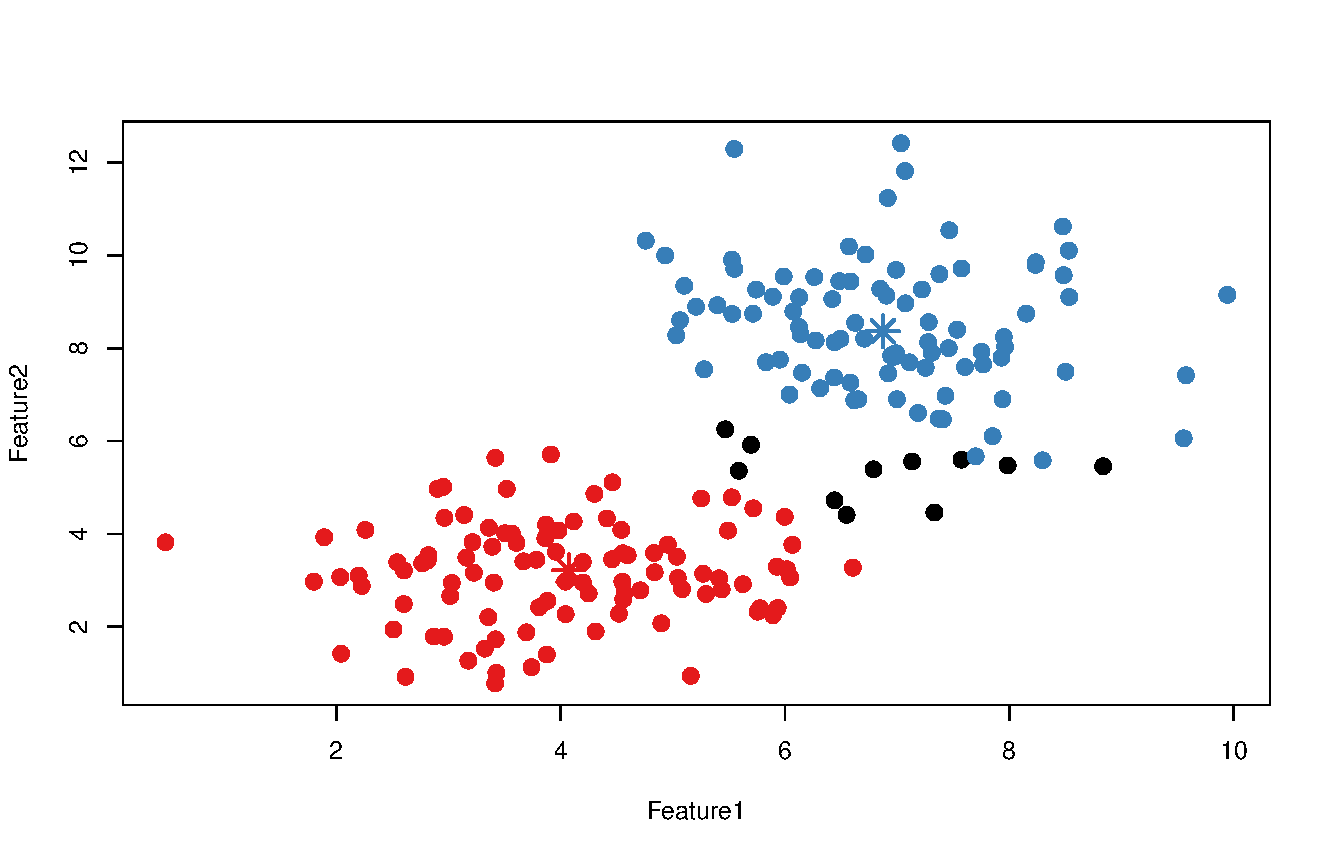
\includegraphics[width=\textwidth]{DemoDataC2D2a_fkm}
		\caption{\textbf{Fuzzy K-Means}}
		\label{fig:DemoDataC2D2a_fkm}
	\end{subfigure}
	\begin{subfigure}[h]{0.49\textwidth}
		\centering
		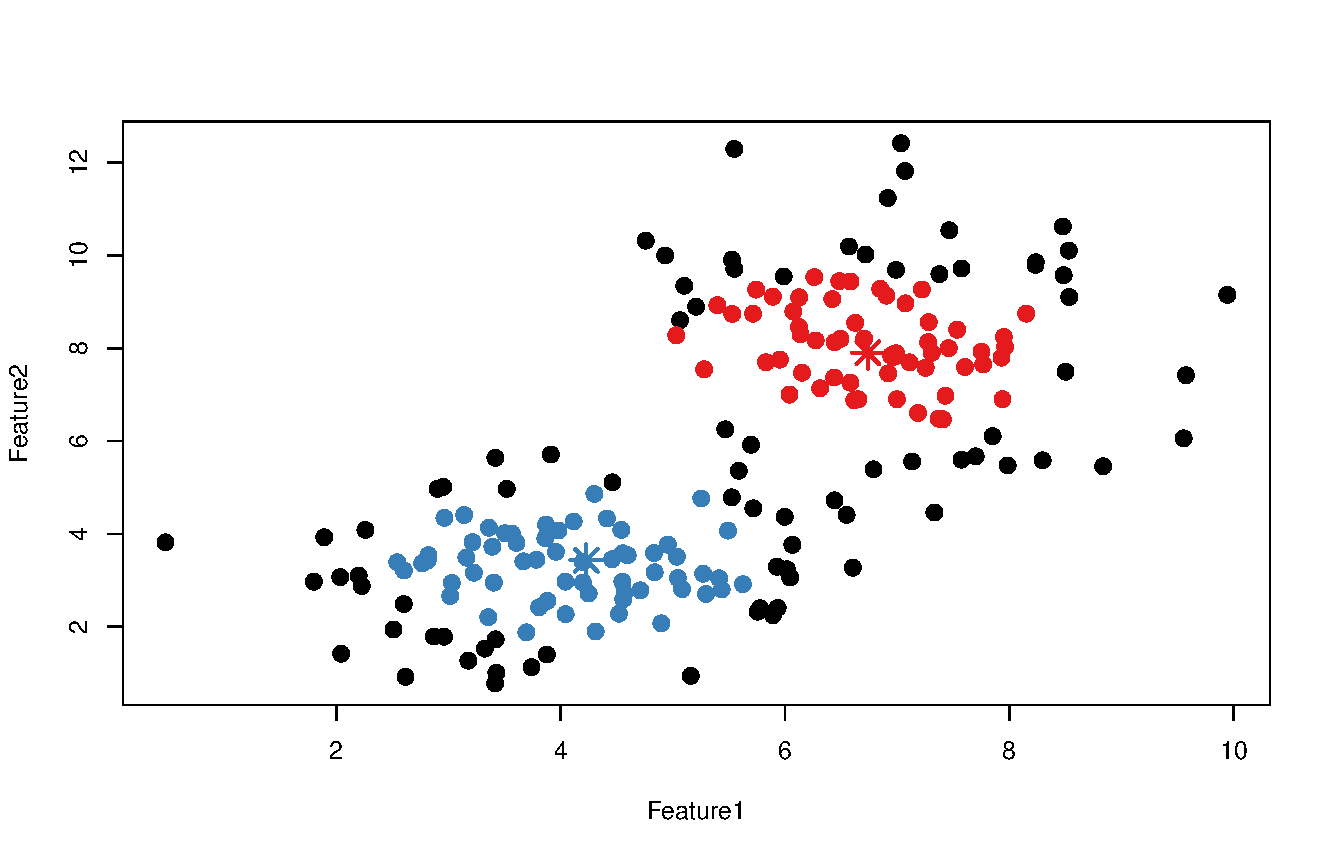
\includegraphics[width=\textwidth]{DemoDataC2D2a_pcm}
		\caption{\textbf{Possibilistic K-Means}}
		\label{fig:DemoDataC2D2a_pcm}
	\end{subfigure}
	\begin{subfigure}[h]{0.49\textwidth}
		\centering
		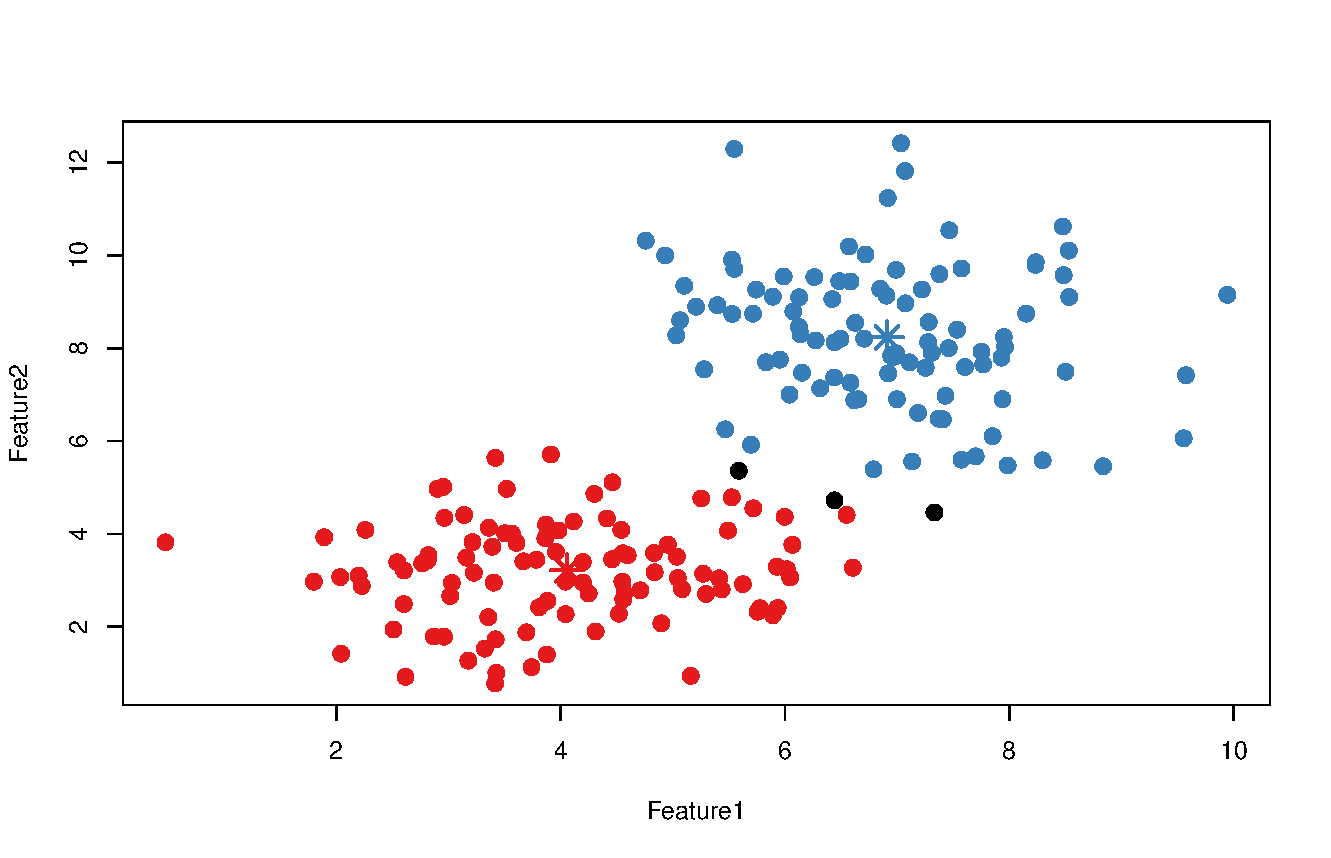
\includegraphics[width=\textwidth]{DemoDataC2D2a_mclust}
		\caption{\textbf{Finite Mixture Gaussian Model}}
		\label{fig:DemoDataC2D2a_mclust}
	\end{subfigure}
	\begin{subfigure}[h]{0.49\textwidth}
		\centering
		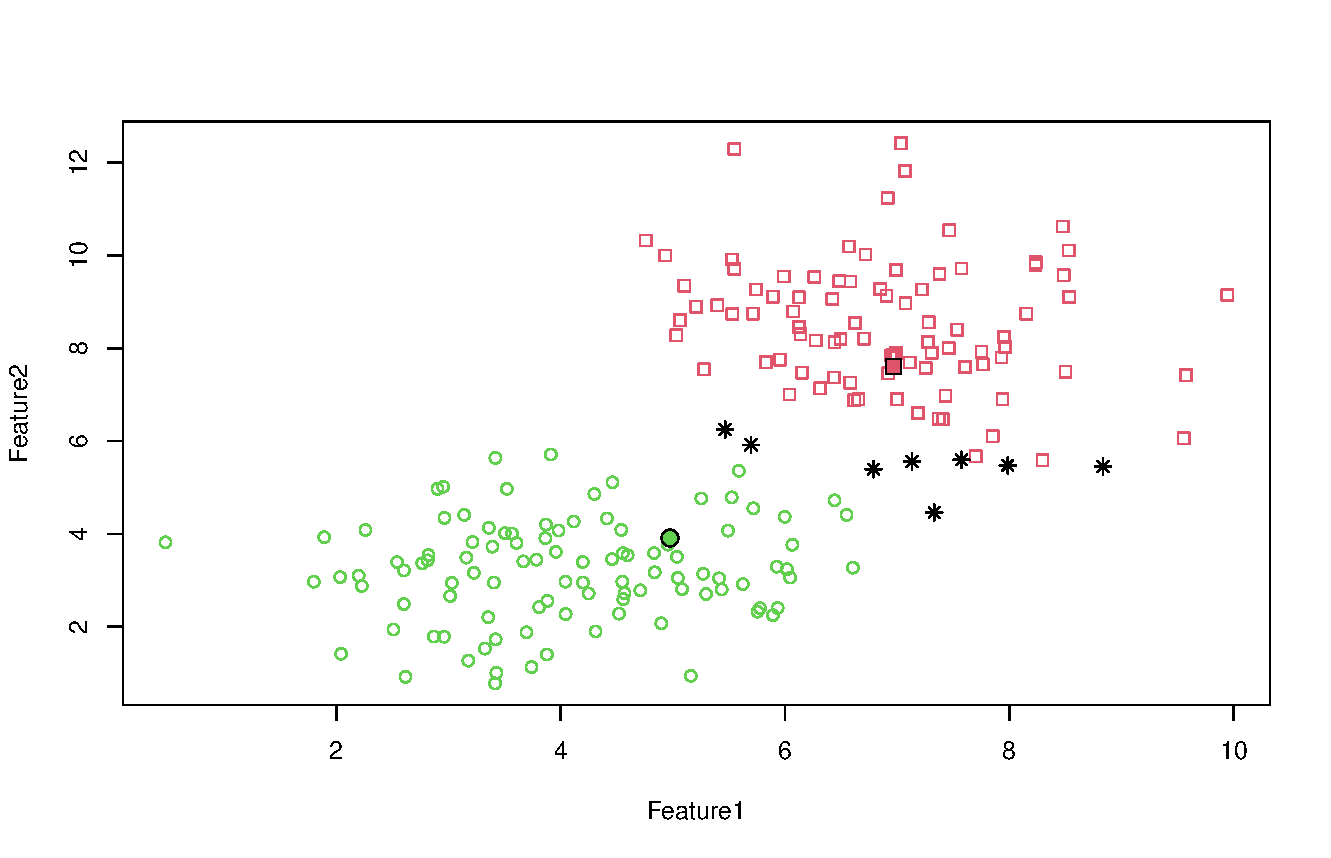
\includegraphics[width=\textwidth]{DemoDataC2D2a_rkm}
		\caption{\textbf{Rough K-Means}}
		\label{fig:DemoDataC2D2a_rkm}
	\end{subfigure}
	\caption{Clustering del Dataset \textit{DemoDataC2D2a}}
	\label{fig:DemoDataC2D2a}
\end{figure}

Nella Figura \ref{fig:DemoDataC2D2a} vengono riportati i risultati dei clustering ottenuti sul dataset \textit{DemoDataC2D2a} usando i colori blu e rosso per differenziare gli oggetti assegnati a cluster diversi e utilizzando il colore nero per quelli oggetti che hanno gradi di appartenenza inferiori a 0.7 nel caso del FkM, oggetti con valori di tipicità inferiori a 0.5 per il PkM, oggetti con probabilità a posteriori inferiori a 0.7 per l'FMG e oggetti in entrambi le UA dei due cluster per il RkM, in altre parole con il colore nero sono rappresentate le partizioni \textit{soft} del clustering. Come possiamo vedere, per il FkM la maggior parte degli oggetti ha dei gradi di appartenenza superiori allo 0.7 e mostra un clustering abbastanza simile a quello del RkM dove solo una piccola parte degli oggetti appartiene ad entrambe le UA dei cluster. Il PkM è quello che ottiene il clustering più diverso per via di come funziona l'algoritmo e per come sono interpretate le appartenenze ai cluster con le tipicità, la maggior parte degli oggetti infatti ha dei gradi di tipicità inferiori allo 0.43. Il FMG invece presenta delle probabilità a posteriori che sono in generale superiori ai gradi di appartenenza e di tipicità dato che solo 3 oggetti presentato probabilità a posteriori inferiori allo 0.7.

I prototipi risultanti sono invece riportati in Tabella \ref{tab:DemoDataC2D2a}. Come si può notare, quelli ottenuti mediante FkM e FMG sono molto simili, mentre quelli ottenuti con RkM sono i più diversi dagli altri. Questo è dovuto al modo in cui sono costruiti, descritto nelle sezioni precedenti.

\begin{table}[h]
	\resizebox{\textwidth}{!}{
		\begin{tabular}{|l|c|c|c|c|c|c|c|c|}
			\hline
			\multicolumn{1}{|c|}{\textbf{}} &
			\multicolumn{2}{c|}{\textbf{FkM}} &
			\multicolumn{2}{c|}{\textbf{PkM}} &
			\multicolumn{2}{c|}{\textbf{FMG}} &
			\multicolumn{2}{c|}{\textbf{RkM}} \\ \cline{2-9} 
			\textbf{} &
			\multicolumn{1}{l|}{Clus 1} &
			\multicolumn{1}{l|}{Clus 2} &
			\multicolumn{1}{l|}{Clus 1} &
			\multicolumn{1}{l|}{Clus 2} &
			\multicolumn{1}{l|}{Clus 1} &
			\multicolumn{1}{l|}{Clus 2} &
			\multicolumn{1}{l|}{Clus 1} &
			\multicolumn{1}{l|}{Clus 2} \\ \hline
			\textbf{Feature 1} & 4.072 & 6.874 & 4.230 & 6.739 & 4.058 & 6.909 & 4.975 & 6.967 \\
			\textbf{Feature 2} & 3.213 & 8.369 & 3.430 & 7.905 & 3.217 & 8.234 & 3.911 & 7.610 \\ \hline
		\end{tabular}
	}
	\caption{Prototipi del Dataset \textit{DemoDataC2D2a}}
	\label{tab:DemoDataC2D2a}
\end{table}

Un discorso molto simile può essere affrontato anche per il clustering del dataset \textit{Synth}, mostrato nella Figura \ref{fig:synth}, dove anche qui vengono confermate le stesse osservazioni fatte prima.

\begin{figure}[h]
	\centering
	\begin{subfigure}[h]{0.49\textwidth}
		\centering
		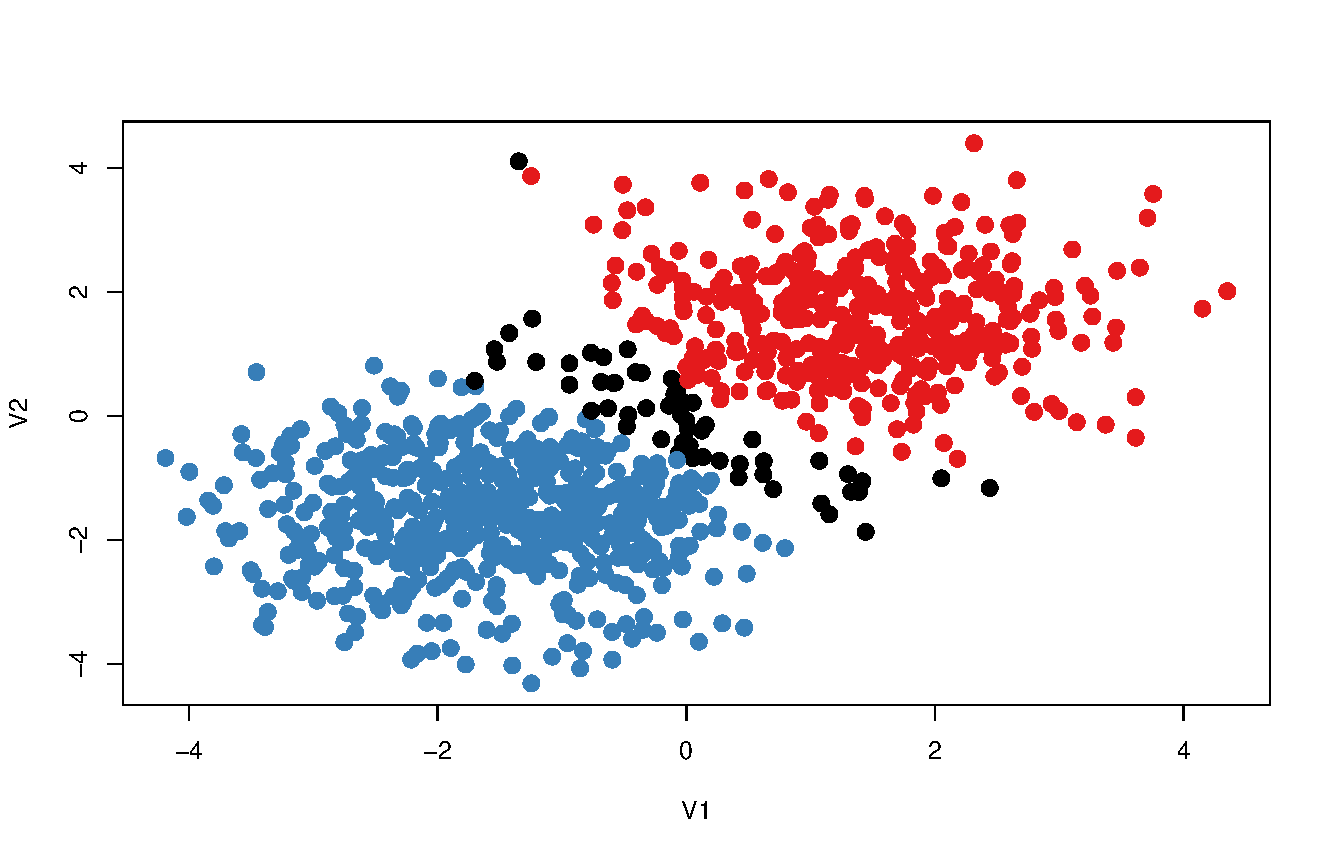
\includegraphics[width=\textwidth]{synth_fkm}
		\caption{\textbf{Fuzzy K-Means}}
		\label{fig:synth_fkm}
	\end{subfigure}
	\begin{subfigure}[h]{0.49\textwidth}
		\centering
		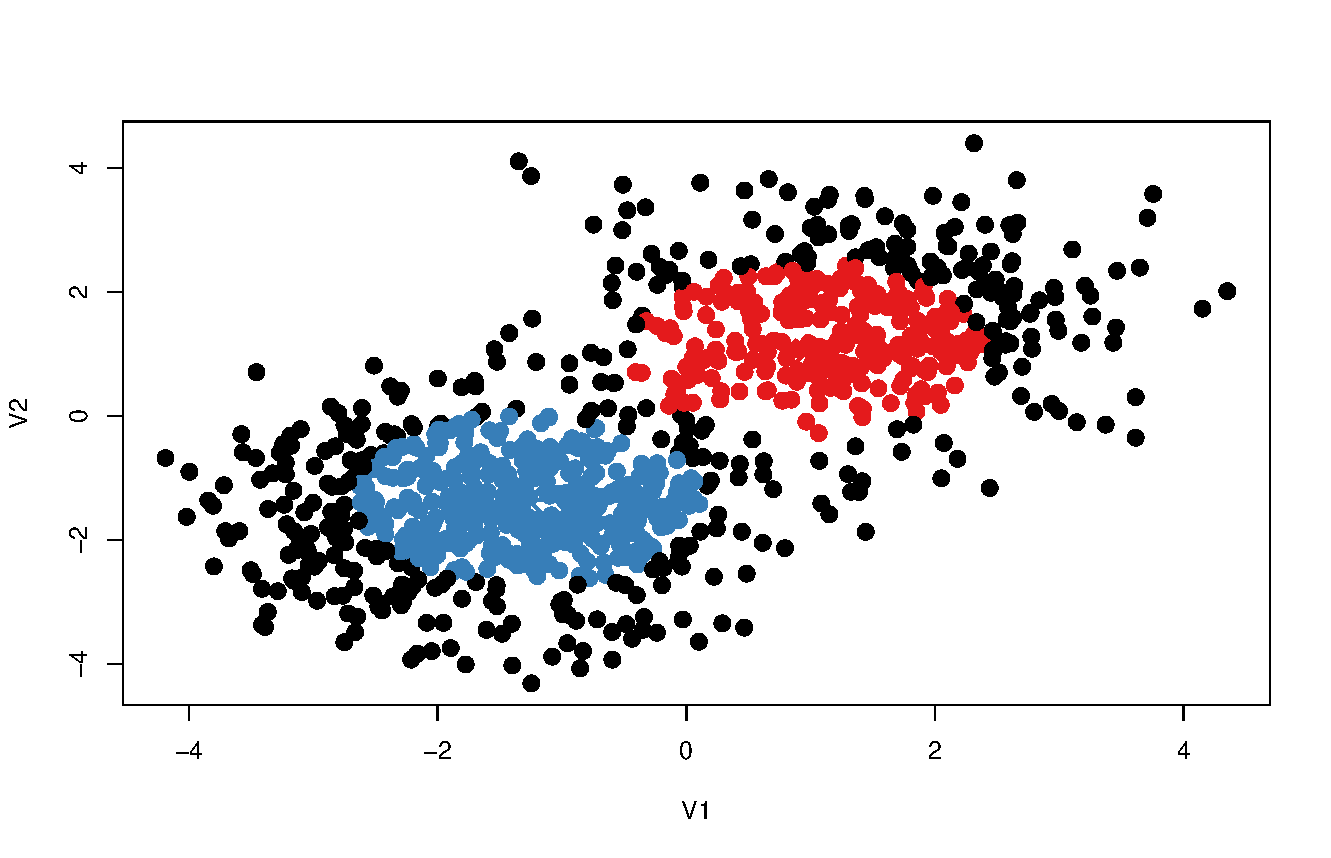
\includegraphics[width=\textwidth]{synth_pcm}
		\caption{\textbf{Possibilistic K-Means}}
		\label{fig:synth_pcm}
	\end{subfigure}
	\begin{subfigure}[h]{0.49\textwidth}
		\centering
		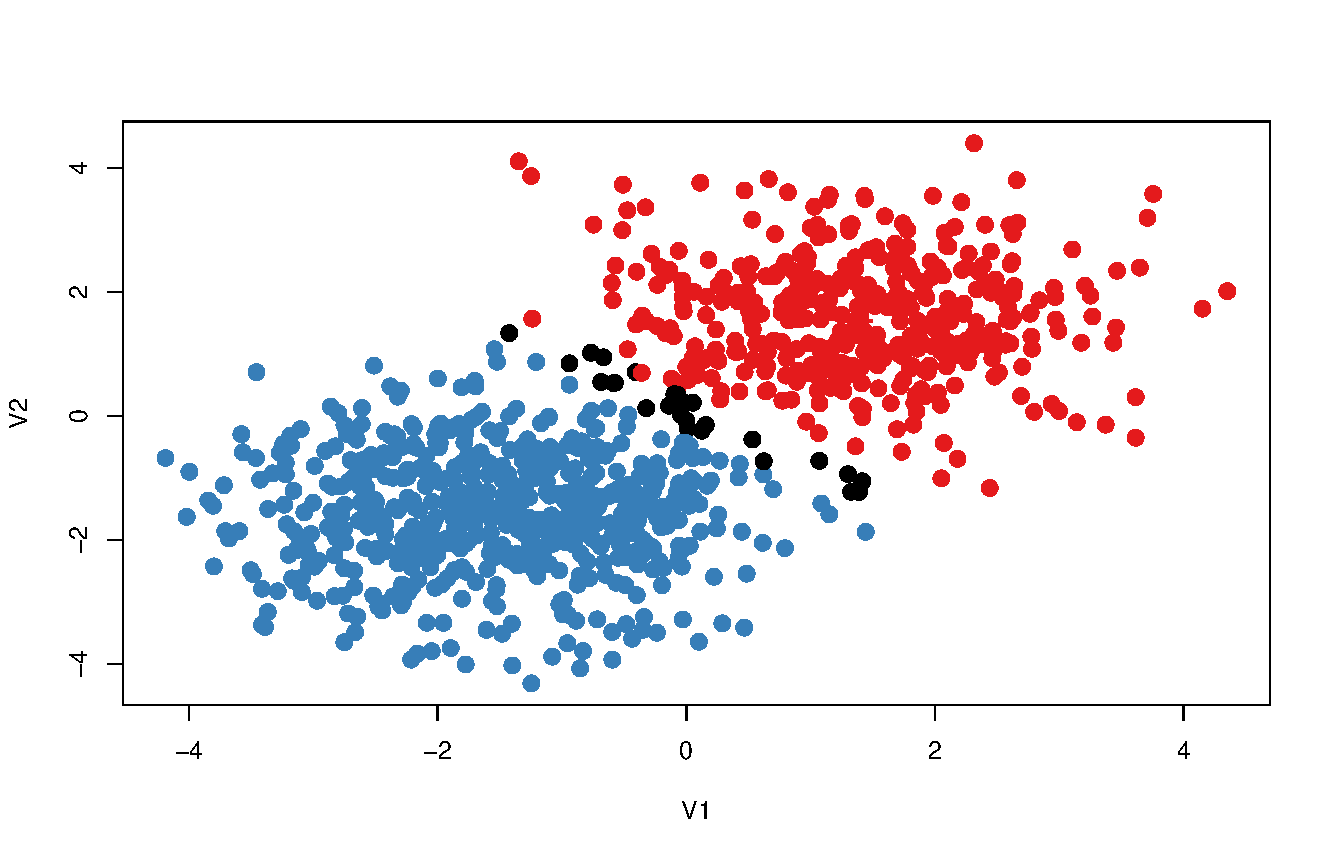
\includegraphics[width=\textwidth]{synth_mclust}
		\caption{\textbf{Finite Mixture Gaussian Model}}
		\label{fig:synth_mclust}
	\end{subfigure}
	\begin{subfigure}[h]{0.49\textwidth}
		\centering
		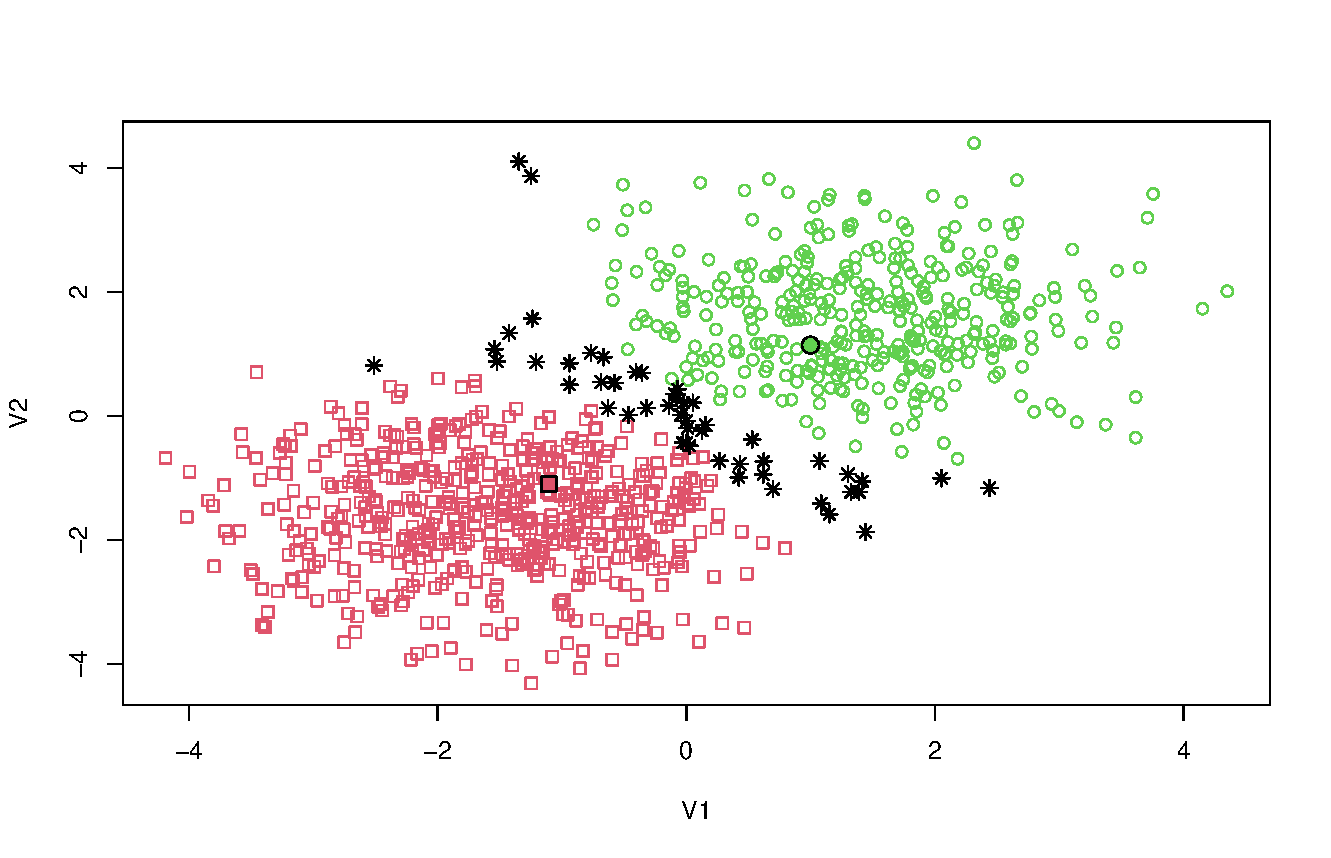
\includegraphics[width=\textwidth]{synth_rkm}
		\caption{\textbf{Rough K-Means}}
		\label{fig:synth_rkm}
	\end{subfigure}
	\caption{Clustering del Dataset \textit{Synth}}
	\label{fig:synth}
\end{figure}

Riportiamo anche i risultati del clustering ottenuti sul dataset \textit{Iris} nella Figura \ref{fig:iris}. Anche in questo caso possiamo vedere come per il FkM abbiamo che la maggior parte degli oggetti hanno gradi di appartenenza superiori allo 0.7, con qualche oggetto più incerto tra il secondo il terzo cluster. Per il PkM invece notiamo come nel dataset dell'\textit{Iris} l'algoritmo incappa nel suo punto debole dei cluster coincidenti, infatti il secondo e il terzo cluster presentano lo stesso centroide e questo si ripercuoterà in seguito sulla valutazione degli indici esterni. L'FMG invece riesce ad ottenere quasi per ogni oggetto delle probabilità a posteriori superiori allo 0.7, distinguendo bene i tre cluster del dataset. Mentre l'RkM riesce a trovare tre cluster ma con centroidi abbastanza diversi rispetto agli altri metodi e con solo una piccola minoranza di oggetti che sono stati associati a tutte e tre le UA dei cluster.

\begin{figure}[h]
	\centering
	\begin{subfigure}[h]{0.49\textwidth}
		\centering
		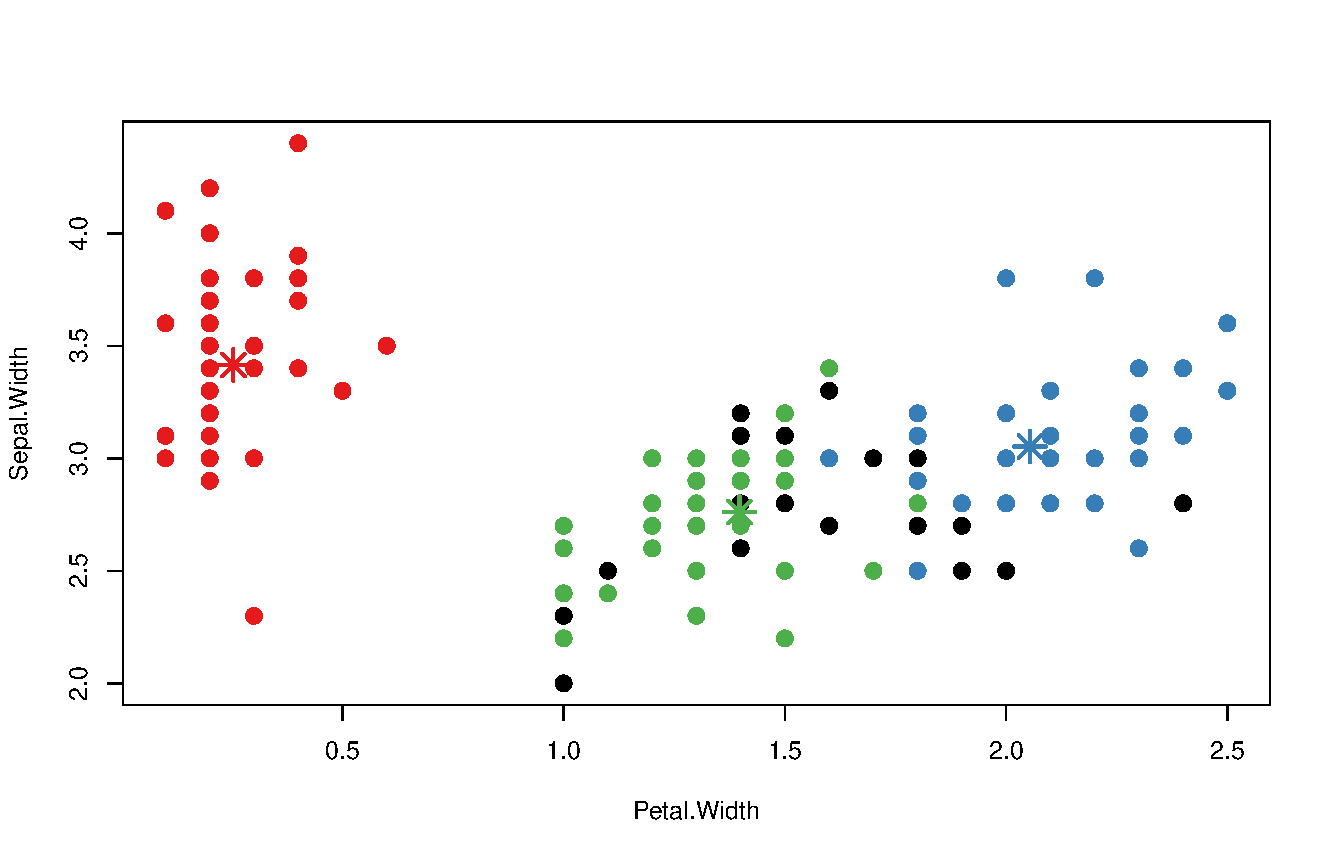
\includegraphics[width=\textwidth]{iris_fkm}
		\caption{\textbf{Fuzzy K-Means}}
		\label{fig:iris_fkm}
	\end{subfigure}
	\begin{subfigure}[h]{0.49\textwidth}
		\centering
		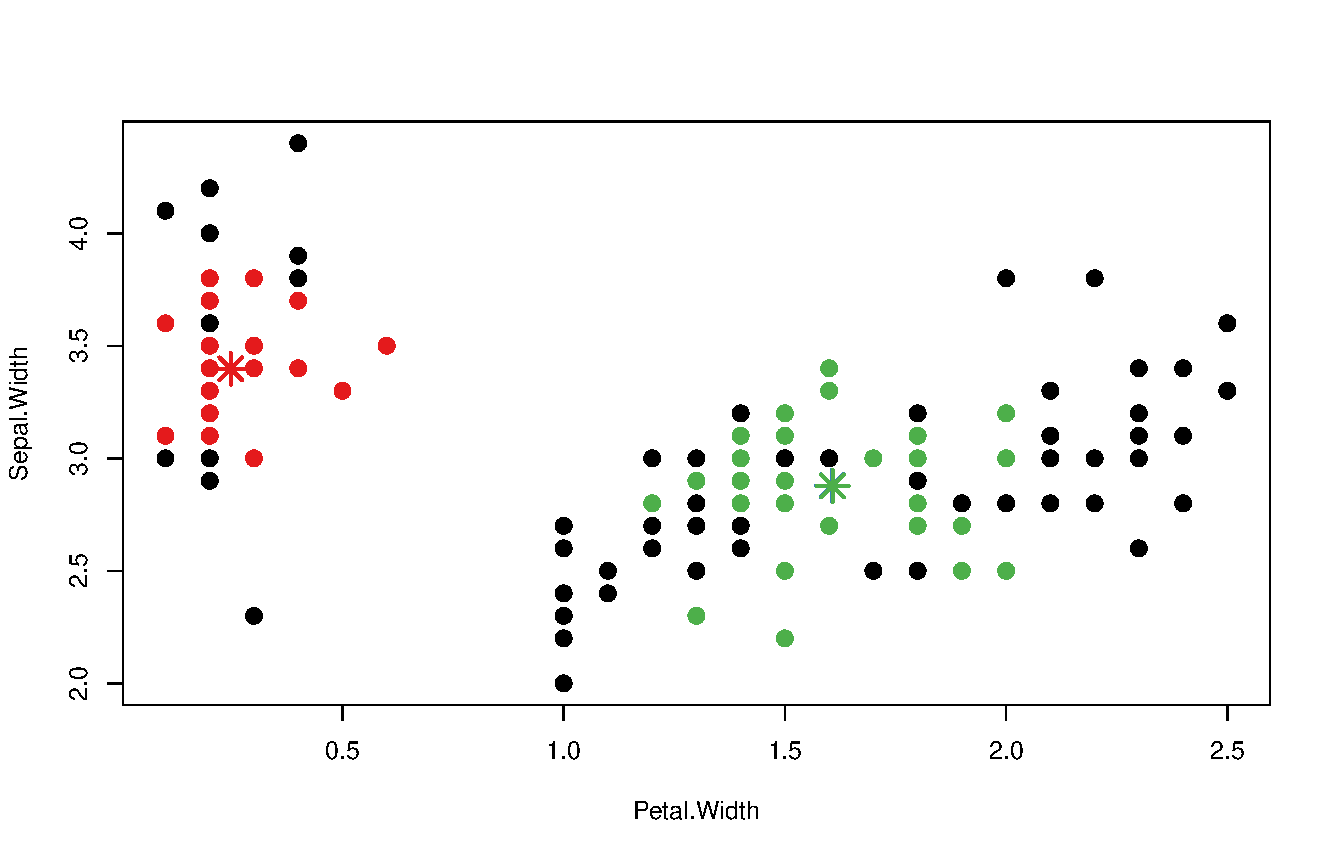
\includegraphics[width=\textwidth]{iris_pcm}
		\caption{\textbf{Possibilistic K-Means}}
		\label{fig:iris_pcm}
	\end{subfigure}
	\begin{subfigure}[h]{0.49\textwidth}
		\centering
		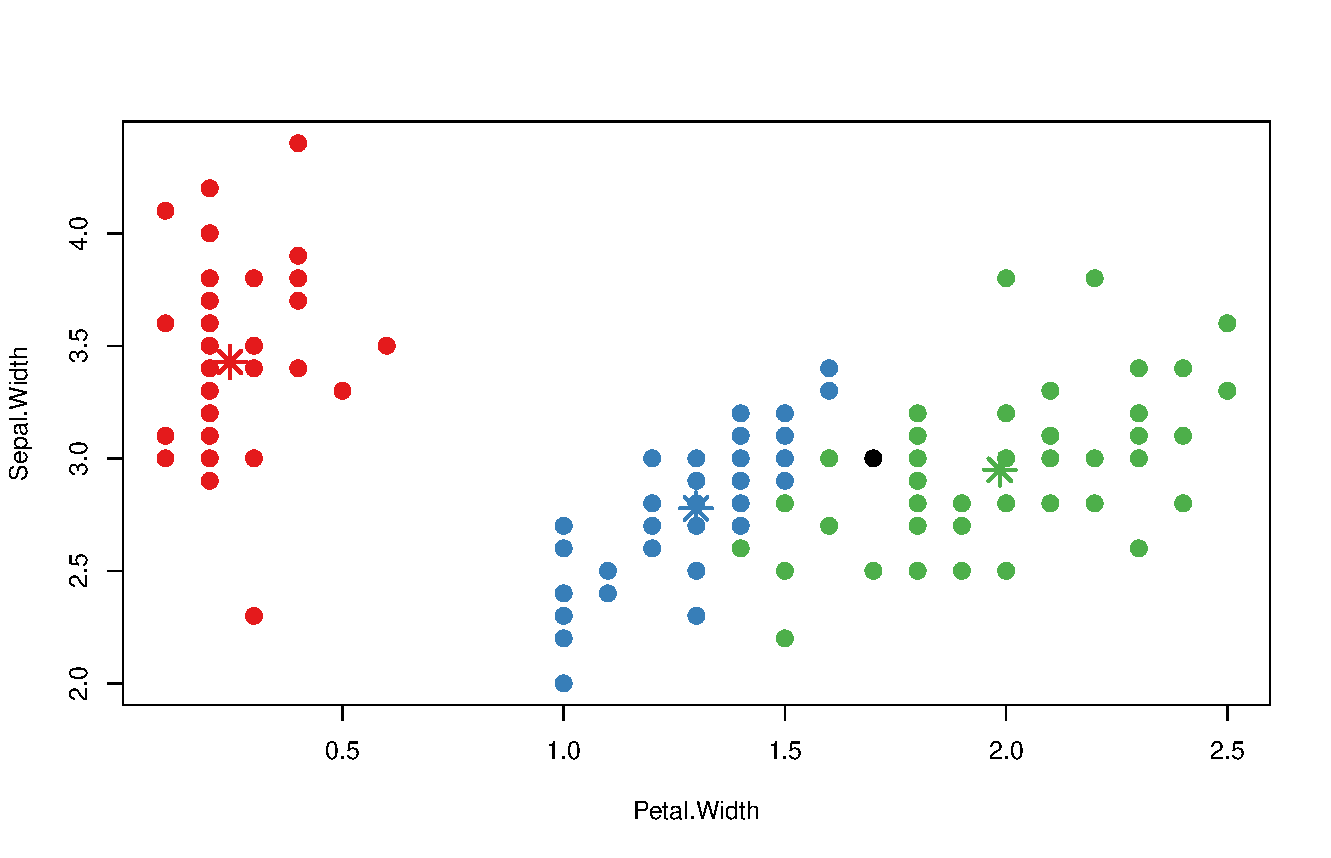
\includegraphics[width=\textwidth]{iris_mclust}
		\caption{\textbf{Finite Mixture Gaussian Model}}
		\label{fig:iris_mclust}
	\end{subfigure}
	\begin{subfigure}[h]{0.49\textwidth}
		\centering
		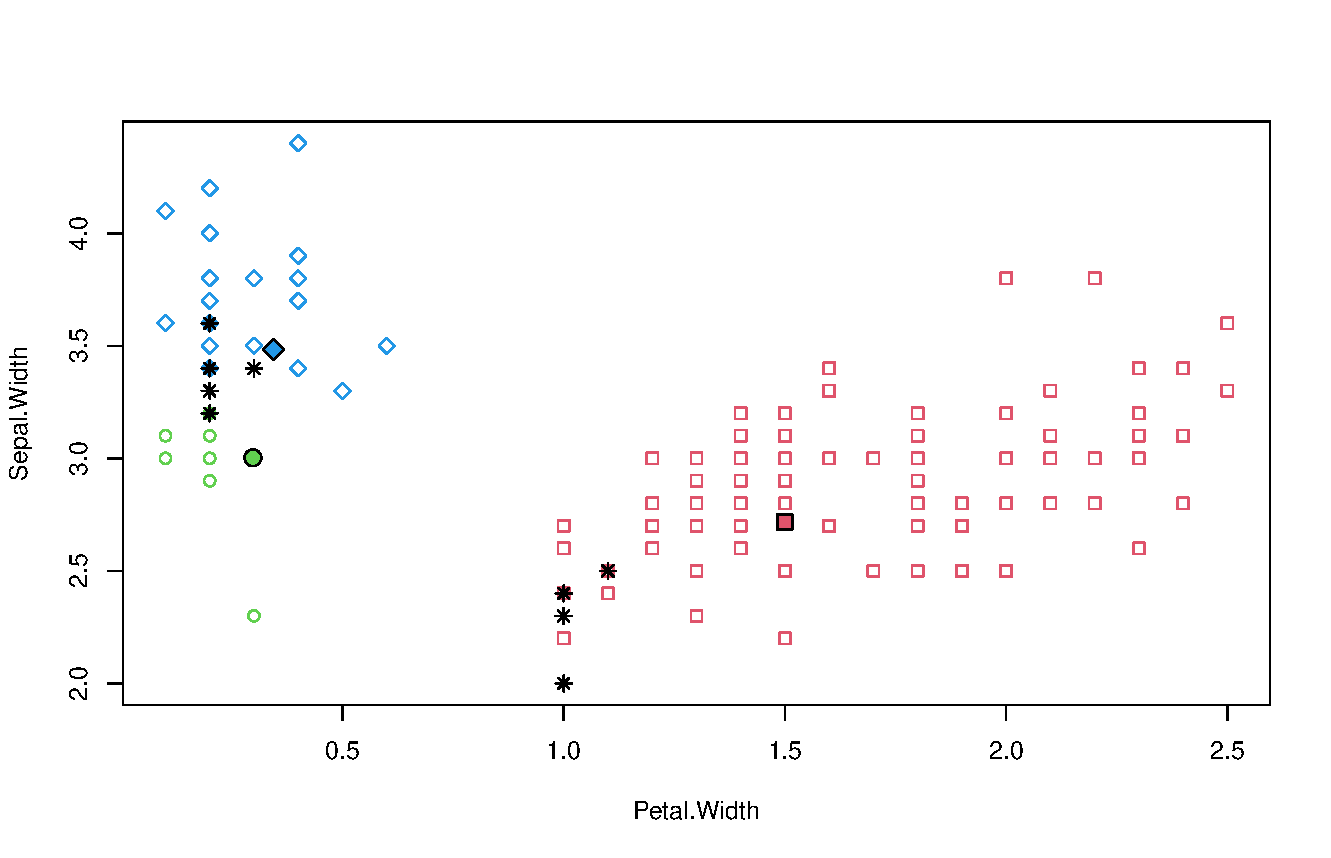
\includegraphics[width=\textwidth]{iris_rkm}
		\caption{\textbf{Rough K-Means}}
		\label{fig:iris_rkm}
	\end{subfigure}
	\caption{Clustering del Dataset \textit{Iris}}
	\label{fig:iris}
\end{figure}

Successivamente riportiamo i risultati ottenuti utilizzando l'indice interno \textit{Fuzzy Silhouette} e gli indici esterni \textit{Purity} e l'\textit{Adjusted Rand Index} (ARI) sul dataset \textit{Iris} rispettivamente nelle Tabelle \ref{fig:fuzzySilhouette} e \ref{tab:externalIris}.

Possiamo notare come l'algoritmo PkM ottiene i valori più alti per il \textit{Fuzzy Silhouette Index} riducendo dunque a generare dei cluster coesi e ben separati fra loro ma comportandosi un po peggio nel caso del dataset \textit{Iris}. Mentre gli altri metodi ottengono comunque dei valori più che soddisfacenti a parte l'FMG sempre nel caso del dataset \textit{Iris}. Per quanto riguarda gli indice esterni invece vediamo come i metodi che si comportano meglio sono l'FkM e l'FMG dato che il PkM come già detto presenta il problema dei cluster coincidenti e nel caso del RkM per via del particolare tipo di partizionamento \textit{soft} che esegue, ma si è voluto comunque provare a interpretare le varie UA come una matrice dei gradi di appartenenza per poterci applicare sopra gli indici precedenti, sia interni che esterni.

Infine vengono riportati i tempi di esecuzione in secondi nella Tabella \ref{tab:execTimes} dove possiamo vedere che in generale l'algoritmo più pesante è il PkM dato che al suo interno riutilizza alcuni valori del FkM come spiegato precedentemente, mentre gli altri metodi su dataset di dimensioni simili a quelli testati hanno tutti tempi di esecuzioni accettabili, il più veloce risulta essere senza sorpresa l'algoritmo più semplice, ovvero, il FkM.

\begin{table}[h]
	\resizebox{\textwidth}{!}{
		\begin{tabular}{|c|c|c|c|c|}
			\hline
			\textbf{- Fuzzy Silhouette Index -} & \textbf{DemoDataC2D2a} & \textbf{G2}     & \textbf{Synth}  & \textbf{Iris}   \\ \hline
			\textbf{Fuzzy K-Means}          & 0.8476 & 0.8525 & 0.8223 & 0.8091 \\
			\textbf{Possibilistic K-Means}      & \textbf{0.8564}        & \textbf{0.8633} & \textbf{0.8230} & \textbf{0.9538} \\
			\textbf{Model-Based Clustering} & 0.8280 & 0.8346 & 0.8038 & 0.6579 \\
			\textbf{Rough K-Means}          & 0.8370 & 0.8388 & 0.8118 & 0.7532 \\ \hline
		\end{tabular}
	}
	\caption{Risultati per il \textit{Fuzzy Silhouette Index}}
	\label{fig:fuzzySilhouette}
\end{table}

\begin{table}[h]
	\centering
	\begin{tabular}{|c|c|c|}
		\hline
		\textbf{- External Indices -} & \textbf{Purity} & \textbf{ARI} \\ \hline
		Fuzzy K-Means                 & 0.9667          & 0.9039       \\
		Possibilistic K-Means         & 0.6667          & 0.5681       \\
		Model-Based Clustering        & 0.9667          & 0.9039       \\
		Rough K-Means                 & 0.5200          & 0.4413       \\ \hline
	\end{tabular}
	\caption{Indici Esterni sul Dataset \textit{Iris}}
	\label{tab:externalIris}
\end{table}

\begin{table}[h]
	\resizebox{\textwidth}{!}{
	\begin{tabular}{|c|c|c|c|c|}
		\hline
		\textbf{- Execution Times -} & \textbf{DemoDataC2D2a} & \textbf{G2} & \textbf{Synth} & \textbf{Iris} \\ \hline
		\textbf{Fuzzy K-Means}          & \textbf{0.0070} & \textbf{0.3590} & \textbf{0.1940} & \textbf{0.0050} \\
		\textbf{Possibilistic K-Means}  & 0.7640 & 5.2400 & 4.7044 & 1.3802 \\
		\textbf{Model-Based Clustering} & 0.0240 & 1.765  & 0.3060 & 0.0680 \\
		\textbf{Rough K-Means}          & 0.1170 & 0.5850 & 0.3500 & 0.0140 \\ \hline
	\end{tabular}
	}
	\caption{Indici Esterni sul Dataset \textit{Iris}}
	\label{tab:execTimes}
\end{table}

\end{document}          
